\documentclass[11pt,a4paper]{article}
\usepackage[margin=2.3cm]{geometry}
\usepackage{enumitem}
\usepackage{titlesec}
\usepackage{hyperref}
\usepackage{xcolor}
\usepackage{booktabs}
\usepackage{parskip}
\usepackage{graphicx}
\usepackage{amsmath}
\usepackage{float}
\usepackage{listings}
\usepackage{tcolorbox}
\tcbuselibrary{listings,breakable,skins}

\definecolor{accent}{RGB}{30,70,120}
\definecolor{green}{RGB}{40,120,40}
\definecolor{red}{RGB}{180,40,40}
\definecolor{codebg}{RGB}{247,247,247}
\definecolor{codeframe}{RGB}{200,200,200}
\definecolor{codekw}{RGB}{0,100,170}
\definecolor{codecomment}{RGB}{100,130,100}
\definecolor{codestr}{RGB}{170,55,55}
\definecolor{strongbg}{RGB}{230,245,230}
\definecolor{strongframe}{RGB}{60,140,60}
\definecolor{warnbg}{RGB}{255,250,230}
\definecolor{warnframe}{RGB}{180,150,40}
\definecolor{failbg}{RGB}{255,235,235}
\definecolor{failframe}{RGB}{180,60,60}

\newtcolorbox{resultbox}[2][]{
    enhanced, colback=#2bg, colframe=#2frame,
    boxrule=0.8pt, arc=3pt, left=6pt, right=6pt, top=4pt, bottom=4pt,
    fonttitle=\bfseries, coltitle=white, title={#1}, breakable,
}

\lstdefinestyle{py}{
    language=Python, basicstyle=\ttfamily\scriptsize,
    keywordstyle=\color{codekw}\bfseries,
    commentstyle=\color{codecomment}\itshape,
    stringstyle=\color{codestr},
    showstringspaces=false, breaklines=true, columns=fullflexible,
    tabsize=4, numbers=left, numberstyle=\tiny\color{gray}, numbersep=8pt,
    frame=leftline, framesep=6pt, rulecolor=\color{codeframe},
    backgroundcolor=\color{codebg}, xleftmargin=14pt,
}
\lstdefinestyle{shell}{
    basicstyle=\ttfamily\scriptsize, commentstyle=\color{codecomment}\itshape,
    showstringspaces=false, breaklines=true, columns=fullflexible, numbers=none,
}
\newtcolorbox{codebox}[1][]{
    colback=codebg, colframe=codeframe, boxrule=0.5pt, arc=2pt,
    left=2pt, right=2pt, top=2pt, bottom=2pt, breakable,
    title={\small\ttfamily #1}, fonttitle=\bfseries\color{accent},
}

\titleformat{\section}{\large\bfseries\color{accent}}{\thesection.\ }{0.4em}{}[\titlerule]
\hypersetup{colorlinks=true, linkcolor=accent, urlcolor=accent}

\begin{document}

\begin{center}
\vspace*{0.4cm}
{\Huge\bfseries\color{accent} The Algorithm}\\[0.8em]
{\Large The complete code behind the\\[0.2em] portfolio comparison}\\[1.4em]
{\small Robin Langer \quad·\quad August 2026}
\end{center}

\vspace{0.6em}

\begin{resultbox}[What this document is]{strong}
One Python file --- \texttt{make\_figure.py}, 247 lines --- that goes
from nothing to the finished diagram: it downloads prices from Yahoo
Finance, computes the momentum signal for all four assets, runs the
capital-recycling rule with the Solana cap, and draws the chart.

\vspace{0.5em}
It is \textbf{self-contained}. It imports no other file in the project.
Copy it onto a bare machine with \texttt{numpy}, \texttt{pandas},
\texttt{matplotlib} and \texttt{yfinance} installed and it reproduces
the diagram from scratch.
\end{resultbox}

\section{What it produces}

\begin{figure}[H]
    \centering
    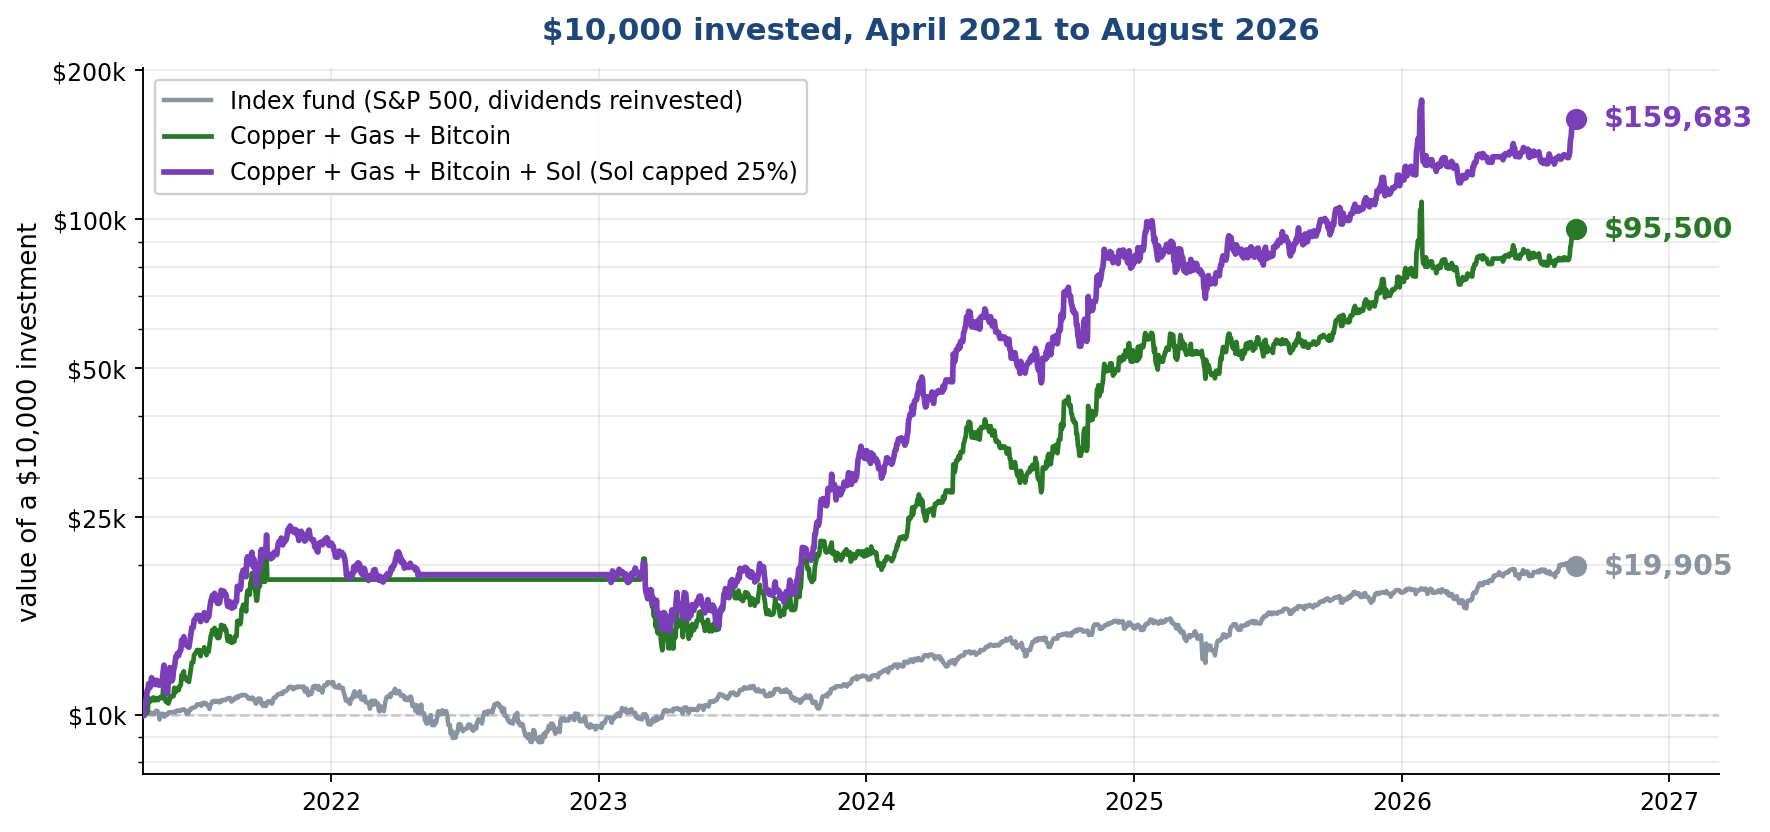
\includegraphics[width=\textwidth]{three_way.png}
\end{figure}

\begin{codebox}[Running it]
\begin{lstlisting}[style=shell]
pip install numpy pandas matplotlib yfinance

python3 make_figure.py                 # writes three_way.png
python3 make_figure.py --cap 0.20      # a different Solana cap
python3 make_figure.py --capital 25000 # a different starting sum
\end{lstlisting}
\end{codebox}

\begin{codebox}[Actual output, run 27 August 2026]
\begin{lstlisting}[style=shell]
Fetching prices and computing momentum (this takes a minute)...

2021-04-19 to 2026-08-26   ($10,000 invested)

  Index fund (S&P 500 total return)   $    19,905    +99%   CAGR 13.7%   worst drop -24.5%
  Copper + Gas + Bitcoin              $    95,500   +855%   CAGR 52.4%   worst drop -35.3%
  + Sol, capped at 25%                $   159,683  +1497%   CAGR 67.8%   worst drop -38.7%

Wrote three_way.png
\end{lstlisting}
\end{codebox}

\section{How it works, in six steps}

\begin{enumerate}[leftmargin=2em, itemsep=5pt]
    \item \textbf{Fetch} (\texttt{fetch}). Daily closes and volumes from
          Yahoo Finance for \texttt{HG=F} (copper), \texttt{NG=F} (gas),
          \texttt{BTC-USD} and \texttt{SOL-USD}, plus
          \texttt{\^{}SP500TR} for the benchmark. Timezones are
          stripped and duplicate dates dropped, so the four series can
          be aligned.

    \item \textbf{Momentum} (\texttt{rolling\_ratio}). For each day,
          weight every daily return in the lookback window by that
          day's volume relative to the window average, then compound
          those flows into a pool seeded at the price at the window's
          start. The pool's final value divided by today's price is the
          \emph{momentum ratio}. Above 1, the weight of money supports a
          higher price.

    \item \textbf{Weights} (\texttt{weights\_for}). Split the money
          equally between whichever assets have a ratio above 1, then
          cap Solana at 25\% and push the excess onto the other active
          assets --- or leave it in cash if there are none.

    \item \textbf{Align} (\texttt{build\_panel}). Crypto trades seven
          days a week, futures do not. The crypto calendar is treated as
          master and futures closes forward-filled onto non-trading
          days, so a held position persists across a weekend at zero
          return.

    \item \textbf{Run} (\texttt{run}). Multiply weights by returns, sum
          across assets, compound. Called twice: once with
          \texttt{cap=0}, which excludes Solana entirely and gives the
          three-asset portfolio, and once with \texttt{cap=0.25}.

    \item \textbf{Draw}. Three lines on a logarithmic axis, each
          labelled with its final value.
\end{enumerate}

\section{Three details that matter}

\begin{resultbox}[The one-day lag]{warn}
\texttt{build\_panel} ends each signal with \texttt{.shift(1)}. Without
it the backtest would buy using a closing price it could not have known
at the time --- the single most common way a backtest invents
returns that were never available. One line, and it is the difference
between a simulation and a fantasy.
\end{resultbox}

\begin{resultbox}[The benchmark includes dividends]{warn}
\texttt{BENCHMARK = "\^{}SP500TR"} is the S\&P 500 \emph{total return}
index, with dividends reinvested. The plain price index
(\texttt{\^{}GSPC}) would have returned $+107\%$ over this period
instead of $+125\%$ --- so using it would have flattered the strategy by
about 18 points it has not earned. If you are going to lose to a
benchmark, lose to the honest one.
\end{resultbox}

\begin{resultbox}[cap=0 is not a special case]{strong}
The three-asset portfolio is not separate code. It is the same function
called with \texttt{cap=0.0}, which forces Solana's weight to zero and
redistributes it. That guarantees the two lines on the chart differ by
\emph{exactly one parameter} --- so the gap between them is the effect
of adding Solana, and nothing else.
\end{resultbox}

\section{The complete listing}

\lstinputlisting[style=py]{portfolio/make_figure.py}

\vspace{1em}

\begin{resultbox}[Verification]{strong}
The momentum arithmetic in \texttt{rolling\_ratio} was checked against
the original \texttt{momentum\_single.py} on identical data:
\textbf{maximum difference 0.000e+00 across 1{,}584 days, and 100\%
agreement on the hold/cash signal.} It is the same algorithm, not a
paraphrase of it.
\end{resultbox}

\begin{resultbox}[]{warn}
\begin{center}
\large\bfseries Historical returns do not guarantee future returns.
\end{center}
\vspace{0.2em}
\centering
This code simulates trades at daily closing prices with no fees,
spread, slippage or tax. Live results will be lower.
\end{resultbox}

\end{document}
